% !TeX root = ../sustechthesis-example.tex

\chapter[用于离子阱量子计算的RTMQ测控系统]{用于离子阱量子计算的RTMQ测控系统\label{section:fpga_rtmq}}

% \textcolor{red}{
% 这部分参考RTMQ的相关专利和文档介绍整个测控系统的情况... 
% }

测控系统能将离子阱量子计算系统中的电学、光学、真空等其余各个部分联系起来,在离子阱量子计算中占据十分重要的地位。量子计算系统的实现涉及到大量物理量的精确调控和测量,这既包括数值上的精确性,也包括时间上的精确性。因此系统对测量和控制性能提出了很多新的要求,其中十分关键的一点就是对测控系统实时性和可拓展性的要求。

传统测控系统以及早些年开发的量子测控系统逐渐难以适应日益增高的量子测控需求,为此本章引入了一种强实时、可拓展、分布式的用于量子物理实验的实时微系统(Real Time Microsystem for Quantum physics, RTMQ),作为后续离子量子计算应用实现的测控系统架构。
接下来的几小节将给出为解决量子物理实验需求专门设计的RTMQ测控系统架构说明,接着阐述与之配套的指令集与时序控制结构描述和节点间用于实时通信的链路系统并给出应用实例,为后续章节内容建立基础。



% % ============================================================================
% % ============================================================================
% % =======================  RTMQ实时量子测控系统 ===============================
% % ============================================================================
% % ============================================================================

\section[RTMQ实时量子测控系统]{RTMQ实时量子测控系统\label{section:rtmq_structure}}

相对于传统测控应用领域,对于离子阱量子计算研究来说,一种实时性更强、可拓展性更好、更灵活的测控系统十分重要。为了满足离子量子计算当前以及未来的测控需求,我们提出了一种实时性可拓展性好、具有分布式计算能力的量子测控系统架构——RTMQ(用于量子物理实验的实时微系统,Real Time Microsystem for Quantum physics)。RTMQ提供了一种新的量子物理实验平台实时测控系统架构,为量子计算的实现提供更好的测控支持。在RTMQ中,通用计算和时序控制由同一微处理器实现,因此避免了两个独立的模块之间同步性的问题;同时树状结构的系统中每个节点都具有通用计算的能力,因此可以实现计算任务的分布式处理,避免了拥塞的问题\cite[]{junhua01}。接下来两小节将介绍RTMQ的测控系统架构及其节点内部结构。


\subsection[RTMQ实时量子测控系统架构]{RTMQ实时量子测控系统架构\label{section:rtmq_architecture}}

\begin{figure}
    \centering
    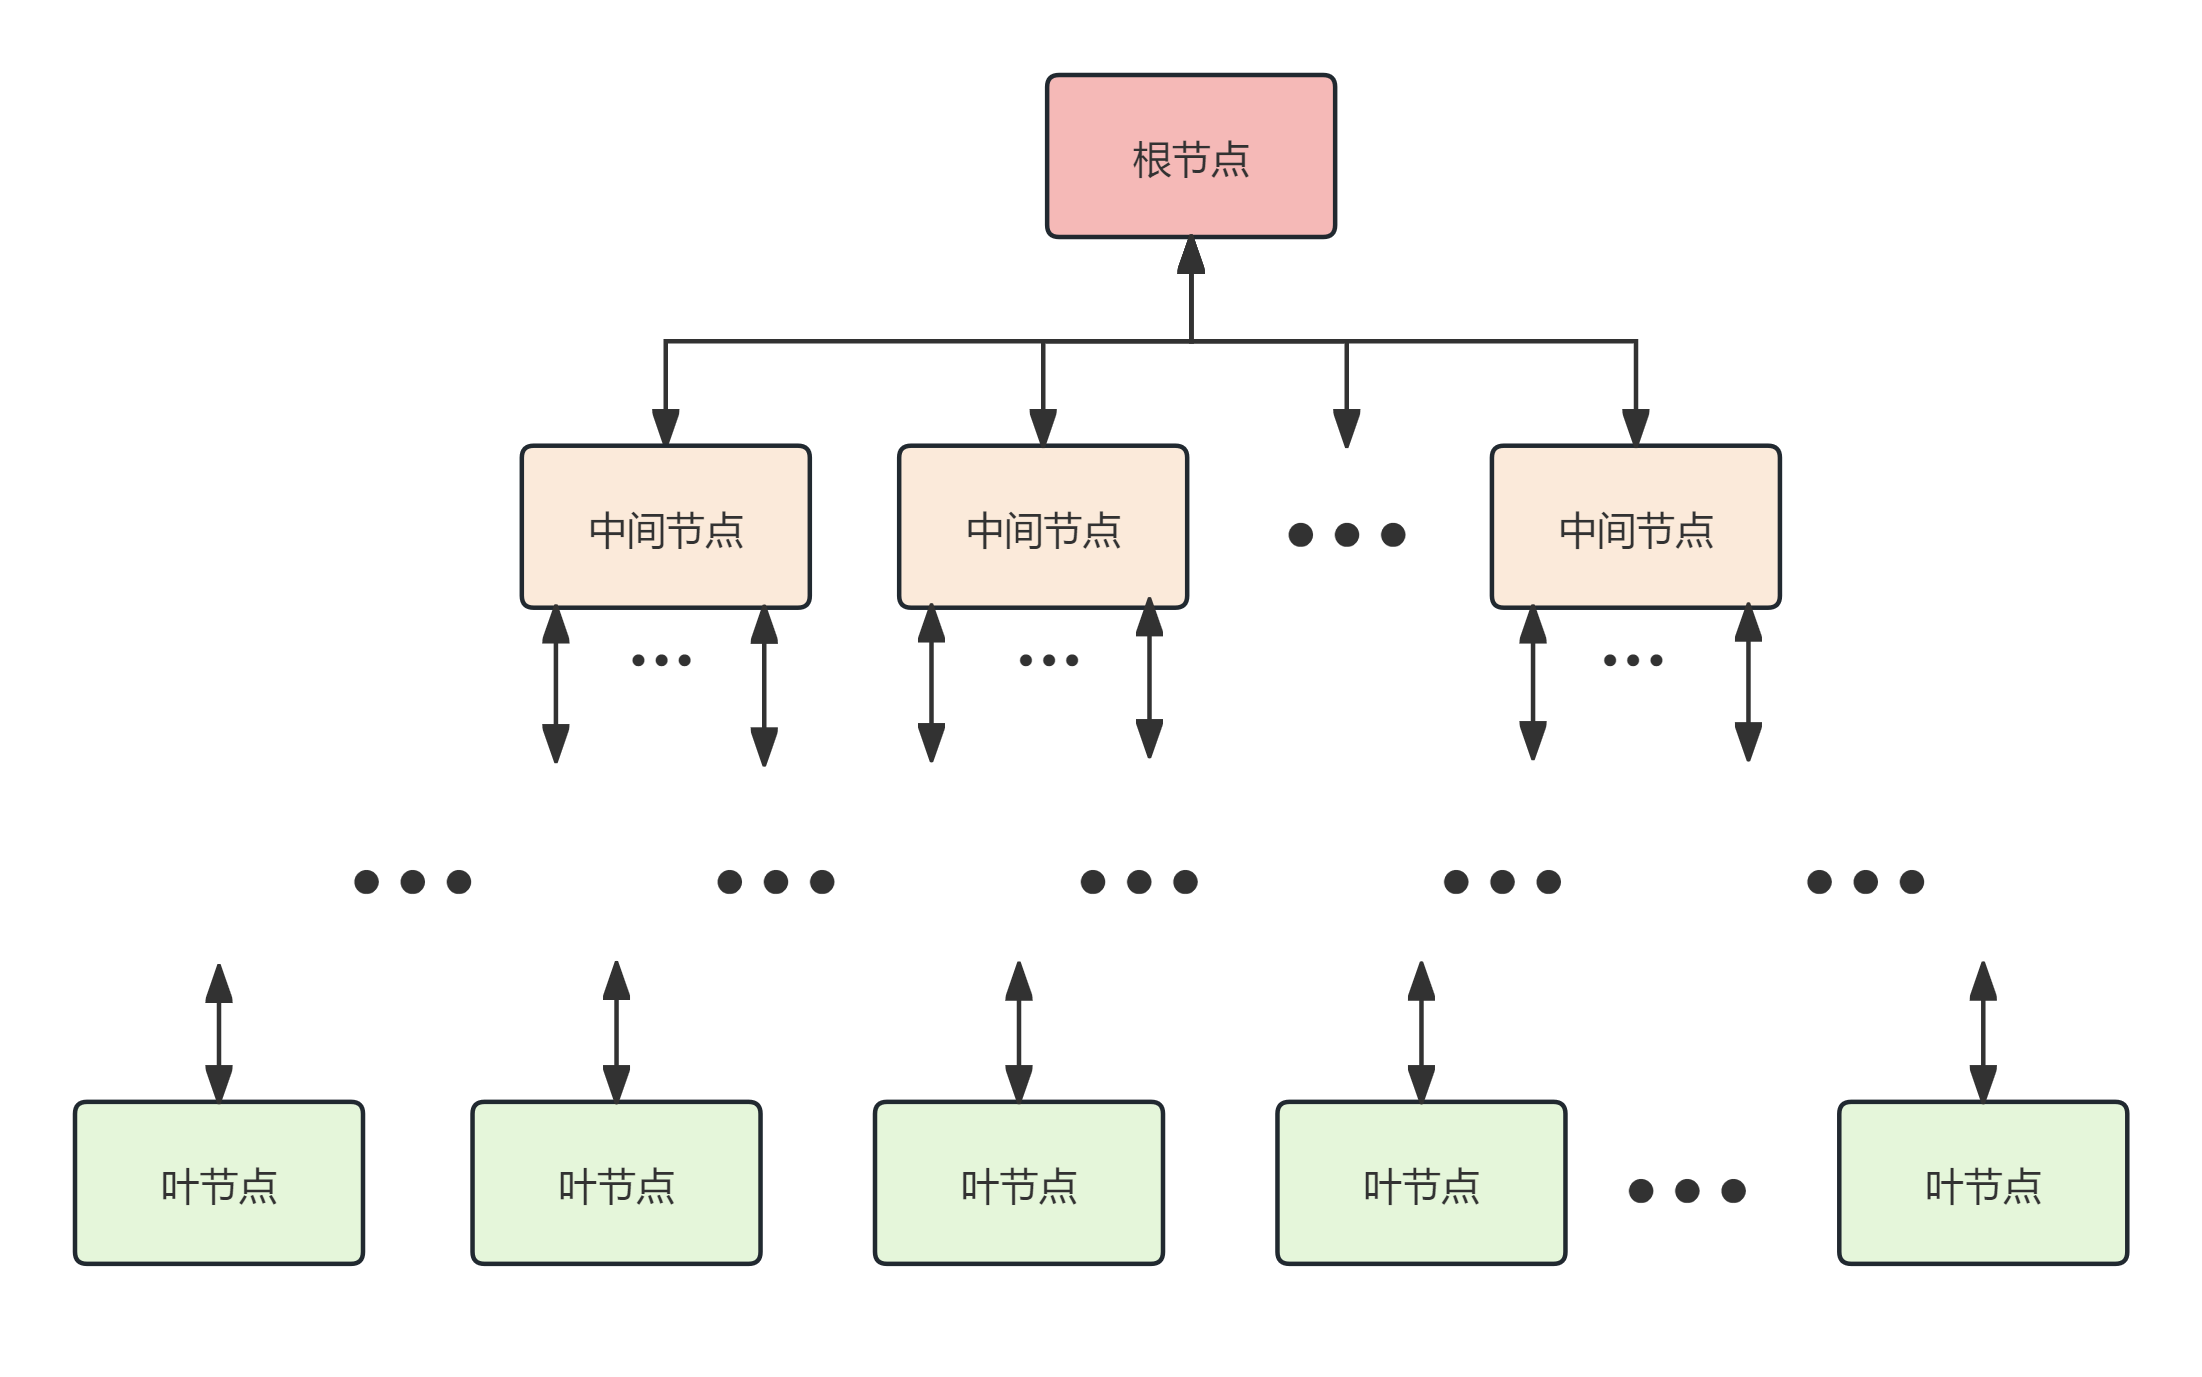
\includegraphics[width=0.9\linewidth]{rtmq/rtmq_nodes_and_leaves_structure}
    \caption[RTMQ实时量子测控系统架构示意图]{RTMQ实时量子测控系统架构示意图\label{fig:rtmq_nodes_and_leaves_structure}}
\end{figure}

RTMQ架构主要用于开发基于FPGA或ASIC的兼具通用计算和高精度时序控制能力的微系统。系统的整体结构为树状结构,如图\ref{fig:rtmq_nodes_and_leaves_structure},系统包含一个根节点,多个中间结点和多个叶节点;根节点通过网络、USB等方式与控制计算机相连。
不同节点的时钟通过根节点进行对齐,各个节点都具有独立的控制输出和通用运算能力,能够分布式地完成实验的控制和信息处理。

\begin{figure}
    \centering
    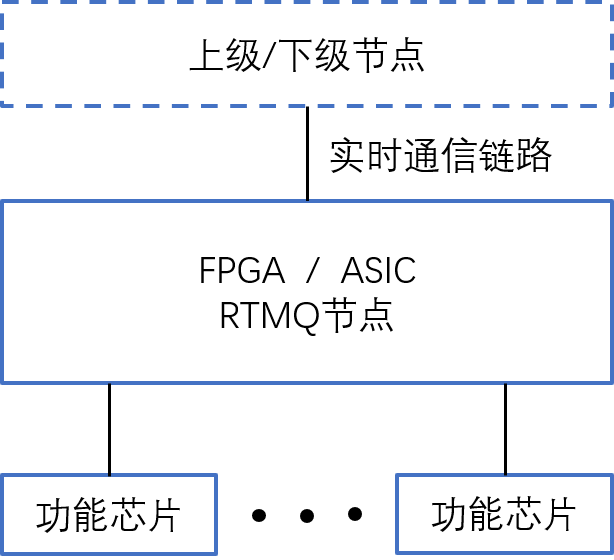
\includegraphics[width=0.6\linewidth]{rtmq/rtmq_board_overal_structure}
    \caption[RTMQ实时量子测控系统架构节点示意图]{RTMQ实时量子测控系统架构节点示意图\label{fig:rtmq_board_overal_structure}}
\end{figure}

各个节点都由测控硬件板卡构成,一般而言一个板卡具有如图\ref{fig:rtmq_board_overal_structure}的结构,板卡上的FPGA或ASIC包含一个RTMQ节点,RTMQ节点通过控制FPGA或ASIC的输入输出与数模/模数转换等各类功能芯片进行交互以实现所需功能,同时通过实时通信链路与其上级和下级节点连接。



\subsection[RTMQ实时量子测控系统架构的节点内部模块]{RTMQ实时量子测控系统架构的节点内部模块\label{section:rtmq_inner_module}}



一个RTMQ节点的内部模块如图\ref{fig:rtmq_board_inner_structure},包含一个32位的微处理器、一个寄存器文件、一系列外设模块和一个链路管理模块。其中微处理器包含流控制器、计时器、异常管理模块、触发管理模块和算术逻辑单元5个子模块;寄存器文件包含多个寄存器;外设可分为系统外设和功能外设,系统外设包括指令缓存、数据缓存、节点信息只读存储器以及地址栈和数据栈,功能外设用于实现具体的逻辑或时序功能。

\begin{figure}
    \centering
    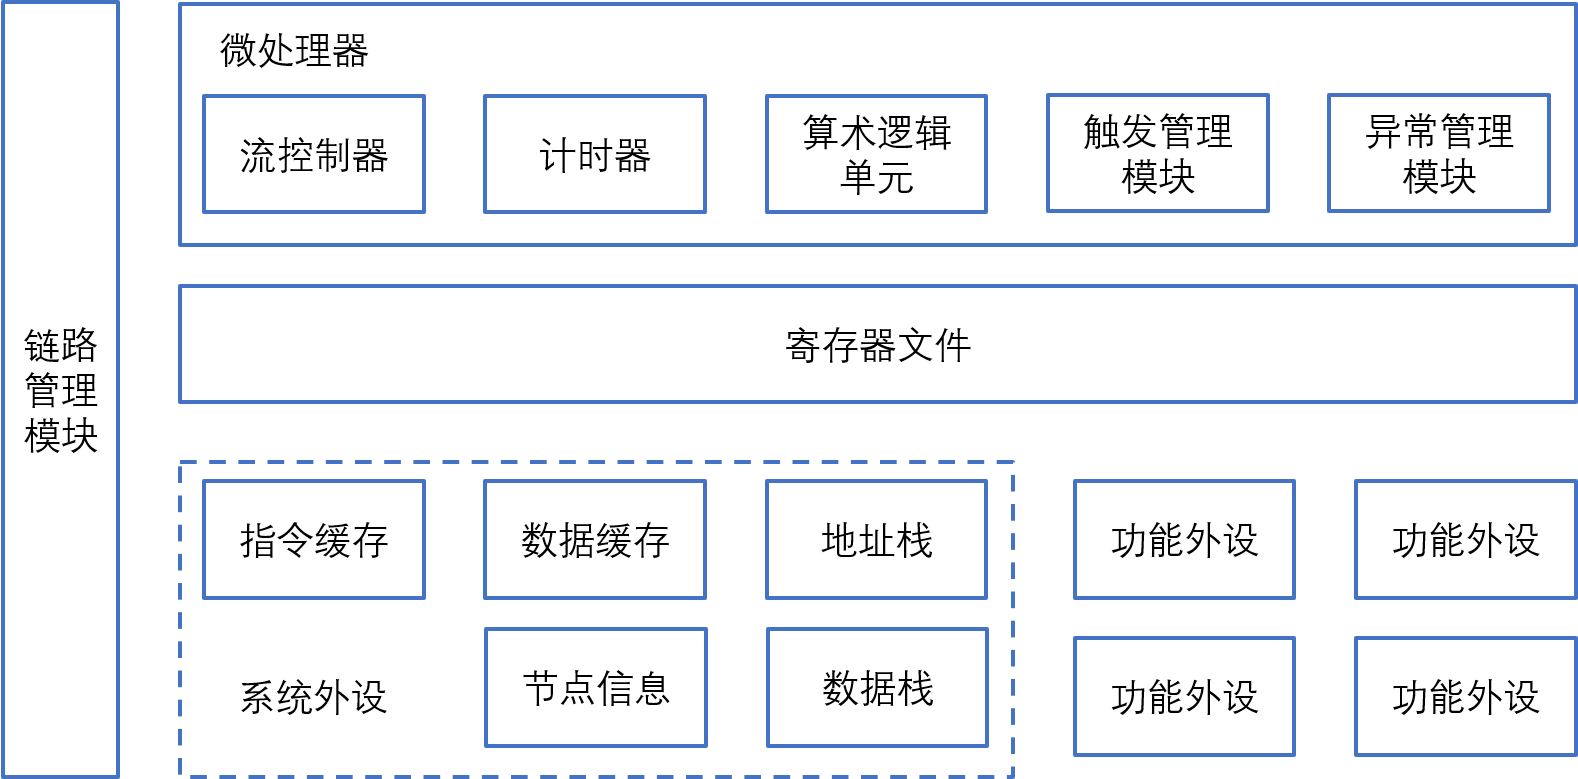
\includegraphics[width=1.0\linewidth]{rtmq/rtmq_board_inner_structure}
    \caption[RTMQ实时量子测控系统架构节点内部模块示意图]{RTMQ实时量子测控系统架构节点内部模块示意图\label{fig:rtmq_board_inner_structure}}
\end{figure}

RTMQ架构中包含的微处理器可受指令控制进入挂起状态,而挂起状态可受计时器或触发管理模块的控制恢复正常运行,如此,微处理器的指令流便可以按一定的时间间隔对齐或与外部信号对齐。同时,节点中的系统外设和功能外设的行为受关联寄存器的读写控制,即微处理器的指令与系统各模块的功能和时序有严格的对应关系。因此,该架构可实现实时控制与通用计算在指令流层面的结合。
而配置指令插入中断的机制确保了节点对其下级节点的绝对控制,即使下级节点的微处理器处于挂起状态,依然不受影响。配置指令插入中断配合具有确定通信延迟的实时通信链路系统,即可实现时序确定的跨节点的即时反馈控制。
此外,RTMQ架构中每个节点都具有通用计算和时序控制能力,如此,大多数通用计算和时序生成都可以在叶节点或较近的中间结点完成,对于大规模系统不存在拥塞的问题,具有良好的可扩展性。
% RTMQ与之前离子阱领域常用的ARTIQ测控系统的对比如表\ref{tb:rtmq_artiq},从对比中可见相较于ARTIQ,RTMQ在反馈延迟、分布式算力、节点自主性、ASIC兼容性、跨领域通用性等方面都有着巨大的优越性。

% \begin{table}
%     \centering
%     \caption[RTMQ与ARTIQ对比]{RTMQ与ARTIQ对比\label{tb:rtmq_artiq}}    
%     \begin{tabular}{L{5cm}|C{4cm}|C{4cm}}
%         \toprule
%         指标 & ARTIQ & RTMQ \\
%         \midrule
%         反馈延迟        & 十微秒 & 百纳秒 \\
%         分布式算力      & × & √ \\
%         节点自主性      & × & √ \\
%         底端FPGA兼容性  & √ & √ \\
%         ASIC兼容性      & × & √ \\
%         二次开发能力    & √ & √ \\
%         跨领域通用性    & × & √ \\
%         \bottomrule
%     \end{tabular}
% \end{table}





% % ============================================================================
% % ============================================================================
% % ======================= RTMQ Instruction Set ===============================
% % ============================================================================
% % ============================================================================
% \newpage



\section[RTMQ的指令集与时序控制结构描述]{RTMQ的指令集与时序控制结构描述\label{section:rtmq_instructions}}
RTMQ配套设计了一种可用于实时控制和通用计算的汇编指令集\cite[]{junhua03}。
该指令集在RTMQ微系统架构中,通过对寄存器的读写访问,达成微处理器与其他逻辑功能模块的交互,同时实现计时和流控制等操作,构建出基本的计时任务与非计时任务等时序控制结构。该指令集以及时序控制结构能够将精确时序控制与通用计算能力在指令流层面完美融合,其时序控制的实现能够精准到单个指令的时钟周期。通用计算和流控制操作并不会对关键实时指令的执行时间产生影响,因而适用于诸如量子物理实验系统控制这类对高精度时序控制和通用计算均有着较高需求的领域。
接下来几小节将从指令的定义、指令的汇编语法、指令的编码、指令的执行逻辑、计时任务与非计时任务块结构等方面介绍RTMQ系统所采用的这种指令集与时序控制结构。

\subsection[RTMQ指令集描述]{RTMQ指令集描述\label{section:rtmq_instruction_set}}


与 RTMQ 架构相配套的、能够用于实时控制和通用计算的指令集中的指令涵盖了以下几个部分:操作码、挂起标记、目标寄存器、操作数0以及操作数1。在该指令集中,指令主要分为两类:I类指令和A类指令。其中,I 类指令的作用是把操作数0或者操作数1直接写入目标寄存器;而A类指令则是将操作数0和操作数1经过操作码所指定的运算之后的结果写入目标寄存器。


\begin{table}
    \centering
    \caption[I类指令的操作码及其含义]{I类指令的操作码及其含义\label{tb:i_instructions}}
    \begin{tabular}{C{2cm}|C{12cm}}
        \toprule
        操作码 & 指令含义 \\
        \midrule
        LDL & 将指令携带的立即数载入目标寄存器的第19到第 0比特\\
        LDH & 将指令携带的立即数载入目标寄存器的第31到第20比特\\
        \bottomrule
    \end{tabular}
\end{table}

\begin{table}
    \centering
    \caption[A类指令的操作码及其含义]{A类指令的操作码及其含义\label{tb:a_instructions}}
    \begin{tabular}{C{1.3cm}|L{7.5cm}|C{1cm}|C{1cm}|C{2cm}}
        \toprule
        操作码 & 指令含义 & 操作数0取反 & 操作数1取反 & 结果取反 \\
        \hline
        \midrule
        ADD & 算术相加 RD = R0 + R1 & 数值反号 & 数值反号 & 数值反号 \\
        \hline
        AND & 按位逻辑与 RD = R0 \& R1 & 按位取反 & 按位取反 & 按位取反 \\
        \hline
        XOR & 按位逻辑或RD = R0 \| R1 & 按位取反 & 按位取反 & 按位取反 \\
        \hline
        CLU & 无符号小于,R0、R1视为无符号数,若R0 < R1则RD = 0xFFFFFFFF,否则RD = 0 & 数值反号 & 数值反号 & 按位取反 \\
        \hline
        CLS & 有符号小于,R0、R1视为有符号数,若R0 < R1则RD = 0xFFFFFFFF,否则RD = 0 & 数值反号 & 数值反号 & 按位取反 \\
        \hline
        CEQ & 等于,若R0 == R1则RD = 0xFFFFFFFF,否则RD = 0 & 数值反号 & 数值反号 & 按位取反 \\
        \hline
        SGN & 符号相乘,RD = R0 * sign(R1) & 数值反号 & 数值反号 & 不支持 \\
        \hline
        SNE & 条件赋值,当R1 < 0时RD = R0,否则RD不变 & 按位取反 & 数值反号 & 赋值条件改为R1 ≥ 0 \\
        \hline
        SMK & 掩码赋值,R1[i]为1时RD[i] = R0[i] ,否则RD[i]不变,Rx[i]代表Rx的第i比特 & 按位取反 & 按位取反 & 不支持 \\
        \hline
        MOV & 赋值,RD = R1 & 无R0 & 按位取反 & 运算结果+1\\
        \hline
        SLL & 逻辑左移,RD = R0 << R1[4:0],R1[4:0]代表R1的最低5比特,若R1 < 0 则为右移,左移时最低位填充R0的最低位,右移时最高位填充0; & 按位取反 & 数值反号 & 右移时最高位填充1 \\
        \hline
        SLA & 算术左移,RD = R0 << R1[4:0],若R1 < 0 则为右移,左移时最低位填充0,右移时最高位填充R0的最高位; & 按位取反 & 数值反号 & 左移时最低位填充1 \\
        \hline
        SLC & 循环左移,RD = R0 << R1[4:0],若R1 < 0 则为右移,移出端移出的比特填充到移入端;& 按位取反 & 数值反号 & 移出的比特按位取反后再填充 \\
        \hline
        REV & 反序,RD[i] = R0[31-i],将R0的二进制位顺序反向,将结果写入RD & 按位取反 & 无R1 & 不支持 \\
        \bottomrule
    \end{tabular}
\end{table}

I类指令的操作码及其含义如表\ref{tb:i_instructions},I类指令用于将立即数写入目标寄存器,仅使用1个立即数作为操作数。A类指令的操作码及其含义如表\ref{tb:a_instructions},A类指令用于执行需要计算的操作,
若操作数属于寄存器,则可以在其别名之前添加取反标记“!”,这意味着先对该操作数进行取反处理,然后再展开计算;目标寄存器的别名之前同样可以添加取反标记,这表示要在运算得出结果之后先进行取反操作,再将其写入目标寄存器;取反操作涵盖了逻辑按位取反、数值反号以及特殊设定的取反操作,不同的指令所采用的取反操作有所差异(其中逻辑按位取反操作指的是针对操作数或者计算结果的每一个位进行逻辑层面的取反;数值反号操作指的是对操作数或者计算结果获取二进制补码)。


当具有挂起标记的指令得以执行时,执行该指令的微处理器会进入挂起状态,从而暂停指令的获取与执行。挂起标记H可以是字符“H”或者“-”。倘若为“H”,则意味着当前指令携带了挂起标记,微处理器在执行这条指令后将进入挂起状态。
此外,指令集中的指令还包含跳转标记,其汇编指令的格式为:
\begin{align}
    OPC \qquad H \qquad F \qquad RD \qquad R0 \qquad R1
\end{align}


其中,OPC代表操作码,H为挂起标记,F为跳转标记,RD为目标寄存器,R0为操作数0,R1为操作数1,操作数可以是寄存器或者立即数。每一个寄存器都对应着一个别名和一个地址,它们分别用于在所述指令集的汇编指令以及机器码中对该寄存器进行指代。跳转标记F可以是字符“F”或者“-”;倘若为“F”,则表明当前指令携带有跳转标记,微处理器在执行这条指令之后将会清空取指流水线。





本文涉及的RTMQ为32位系统,其寄存器的位宽为32位,因此相应指令集的指令编码长度也为32位。指令集的指令编码方案如表\ref{tb:instructions_code},大体有五类情况:LDL、LDH、MOV、REV及其它A类指令。几类情况的共同点为[29-28]位分别为挂起和跳转标志位以及[23-16]位为RD地址,其余各位的编码根据具体的操作而有所不同。
其中,LDL和LDH为I类指令,两者的区别主要在于载入立即数位数的不同。其中LDL会将指令携带的立即数载入目标寄存器的第19到第0比特(20位),而LDH会将指令携带的立即数载入目标寄存器的第31到第20比特(12)位。在A类指令编码中有两个特殊的指令MOV和REV,与其余A类指令每次同时操作R0和R1两个操作数不同,这两个指令操作对象仅为一个操作数(R0或R1)。
% 上面这段是看表补充的

\begin{table}
    \centering
    \caption[指令集的指令编码方案]{指令集的指令编码方案\label{tb:instructions_code}}
    \begin{tabular}{C{1cm}|C{1.5cm}|C{1.5cm}|C{2cm}|C{1cm}|C{5cm}}
        \toprule
         比特 & LDL & LDH & MOV & REV & 其它A类指令 \\
        \midrule
        31      & 1 & 1 & \multicolumn{3}{|c}{0} \\
        \hline
        30      & 1 & 0 & \multicolumn{3}{|c}{目标寄存器RD取反标记,为1则取反} \\
        \hline
        29      & \multicolumn{5}{|c}{挂起标记,为1则当前指令使得微处理器进入挂起状态} \\
        \hline
        28      & \multicolumn{5}{|c}{跳转标记,为1则微处理器清空从指令缓存取指的流水线} \\
        \hline
        27-24   & 立即数19-16位 & 0 & \multicolumn{3}{|c}{操作码} \\
        \hline
        23-16   & \multicolumn{5}{|c}{RD的地址} \\
        \hline
        15      & \multicolumn{2}{|c|}{立即数15位}  & 1 & 0 & 操作数R0立即数标记,为1表示R0为立即数 \\
        \hline
        14      & \multicolumn{2}{|c|}{立即数14位}  & 0 & 1 & R1立即数标记,为1表示R1为立即数 \\
        \hline
        13      & \multicolumn{2}{|c|}{立即数13位}   & 0 & \multicolumn{2}{|C{6cm}}{若R0为寄存器,则为取反标记,为1则取反;若R0为立即数,则为R0的第6位} \\
        \hline
        12      & \multicolumn{2}{|c|}{立即数12位}   & 操作数1取反标记,为1则取反 & 0 & 若R1为寄存器,则为取反标记;若R1为立即数,则为R1的第6位 \\
        \hline
        11-8    & \multicolumn{2}{|c|}{立即数11-8位}   & 0 & R0的地址 & 若R0为寄存器,则为其地址;若R0为立即数,则为其5-0位 \\
        \hline
        7-6     & \multicolumn{2}{|c|}{立即数7-6位}   & R1地址 & 0 & 若R0为寄存器,则为其地址;若R0为立即数,则为其5-0位\\
        \hline
        5-0     & \multicolumn{2}{|c|}{立即数5-0位}   & R1地址 & 0 & 若R1为寄存器,则为其地址;若R1为立即数,则为其5-0位 \\
        \bottomrule
    \end{tabular}
\end{table}


在RTMQ微系统架构当中,包含着能够响应指令相关操作的寄存器的读、写访问进行处理的功能逻辑模块。当RTMQ中的某一寄存器在作为A类指令的操作数而被读取时,和其相关联的上述功能逻辑模块会执行响应读取访问的逻辑功能。当某一寄存器作为A类指令或者I类指令中的LDL指令的目标寄存器而被写入时,与其相关联的上述功能逻辑模块则会执行响应写入访问的逻辑功能。

在RTMQ微系统架构中,存在与寄存器TIM相关联的计时器模块,它可与指令集相互配合。具体而言,当向TIM寄存器进行写入操作时,计时器模块便会启动倒计时,其起始时间计数即为TIM寄存器的写入值;在每个系统时钟周期,时间计数会减1,直至降为0时停止倒计时;倒计时结束之后,倘若该微系统架构中的微处理器处于挂起状态,那么将会解除这一挂起状态。另外,RTMQ中还设有一个别名为NUL、地址为0的寄存器,此寄存器被定义为空寄存器,对其进行写入操作不会产生任何实际效果,而它的读取值始终为0。空指令“NOP H F”被定义为“ADD H F NUL NUL NUL”,其中挂起标记H和跳转标记F能够依据需求进行设定,除此之外,该空指令不会产生其它任何作用。

\subsection[计时任务块与非计时任务块]{计时任务块与非计时任务块}

基于第\ref{section:rtmq_instruction_set}节中所述的指令集和RTMQ计时器模块的逻辑功能,可以定义结合精确时序控制和通用计算的程序结构,称为计时任务块,其结构如表\ref{tb:timed_program1}。在实际实验应用中会存在与所述计时任务块在功能上等价的其它程序结构,包括将挂起标记H向上一条指令或下一条指令移动、利用其它指令写入TIM寄存器等等情况。

\begin{table}
    \centering
    \caption[计时任务块结构]{计时任务块结构\label{tb:timed_program1}}
    \begin{tabular}{C{7cm}|C{7cm}}
        \toprule
        若T为寄存器 & 若T为立即数 \\
        \midrule
        NOP - -& LDH - - TIM T \\
        MOV - - TIM T & LDL - - TIM T \\
        \dots  & \dots \\
        (一条或多条其它指令) & (一条或多条其它指令) \\
        NOP H - & NOP H -\\
        \bottomrule
    \end{tabular}
\end{table}


若在程序中有大计算量的通用计算存在或有等待外触发等执行时间可能不确定的需求,可定义非计时任务块结构,其结构如表\ref{tb:untimed_program}。在实际实验应用中也会存在与“MOV - - TIM NUL”等价的其它激活计时器的短时间倒计时的方式,包括使用“ADD - - TIM NUL NUL”、“LDL - - TIM 0”等功能上等价的指令以及对初始时间计数的调整。

\begin{table}
    \centering
    \caption[非计时任务块结构]{非计时任务块结构\label{tb:untimed_program}}
    \begin{tabular}{C{14cm}}
        \toprule
        NOP H -\\
        (一条或多条其它指令)\\
        MOV - - TIM NUL \\
        \bottomrule
    \end{tabular}
\end{table}










% ============================================================================
% ============================================================================
% ======================     RTMQ Link System   ==============================
% ============================================================================
% ============================================================================
\newpage
\section[RTMQ节点间的实时通信链路系统描述]{RTMQ节点间的实时通信链路系统描述\label{section:rtmq_links}}

RTMQ实时量子测控系统架构具有强大的可拓展性,不同板卡节点之间可以实现完全的实时通信,这种通信的实现依赖于一种专门设计的链路系统。
在该链路系统里,所有节点跟其上级、下级节点之间存在统一、恒定并且较短的通信延迟,这适用于实时控制的场景;而且在链路当中,不仅能够传递数据,还能够传递指令,便于上级节点对下级节点实施实时的控制,从而达成更为复杂的交互功能。

\subsection[RTMQ节点间的实时通信链路系统]{RTMQ节点间的实时通信链路系统}
由RTMQ节点所构成的硬件系统以树状结构进行扩展,节点被划分为根节点、中间结点以及叶节点这三类。根节点和中间结点具备一个或者多个与其直接相连的下级节点,中间结点和叶节点拥有一个与其直接相连的上级节点。在该链路系统中,节点之间直接通信所采用的物理链路协议是具有固定通信延迟、固定最小通信单元长度的双向点对点通信协议,例如UART或者SPI。
RTMQ节点之间的通信是以帧作为单位的,帧涵盖了魔术字、跳转数、帧类型以及载荷这4个数据域。其中,魔术字用于对当前帧的有效性予以验证;跳转数用于指明当前帧能够被转发的次数;帧类型可以是数据帧或者指令帧,其作用是指示当前帧的载荷类型;载荷则是当前帧所携带的有效信息,依据当前帧的帧类型,载荷能够被接收该帧的节点解析成为数据或者指令。
链路管理模块内部逻辑结构如图\ref{fig:rtmq_link_module},一个节点收到的指令帧会被交由微处理器执行,而数据帧则会存放在专门的缓冲区等待微处理器读取。一个节点可以任意的向上级或下级节点发送数据帧,而指令帧仅能向其下级节点发送。除了发送之外,节点还可以向上或向下转发跳转数不为0的帧,从而能实现跨层级的通信。链路管理模块作为重要的外设,其功能同样受到寄存器的控制,包括功能配置寄存器RTCF、广播寄存器RTBC以及一系列对应上级和下级节点通信的收发寄存器RTDx。

\begin{figure}
    \centering
    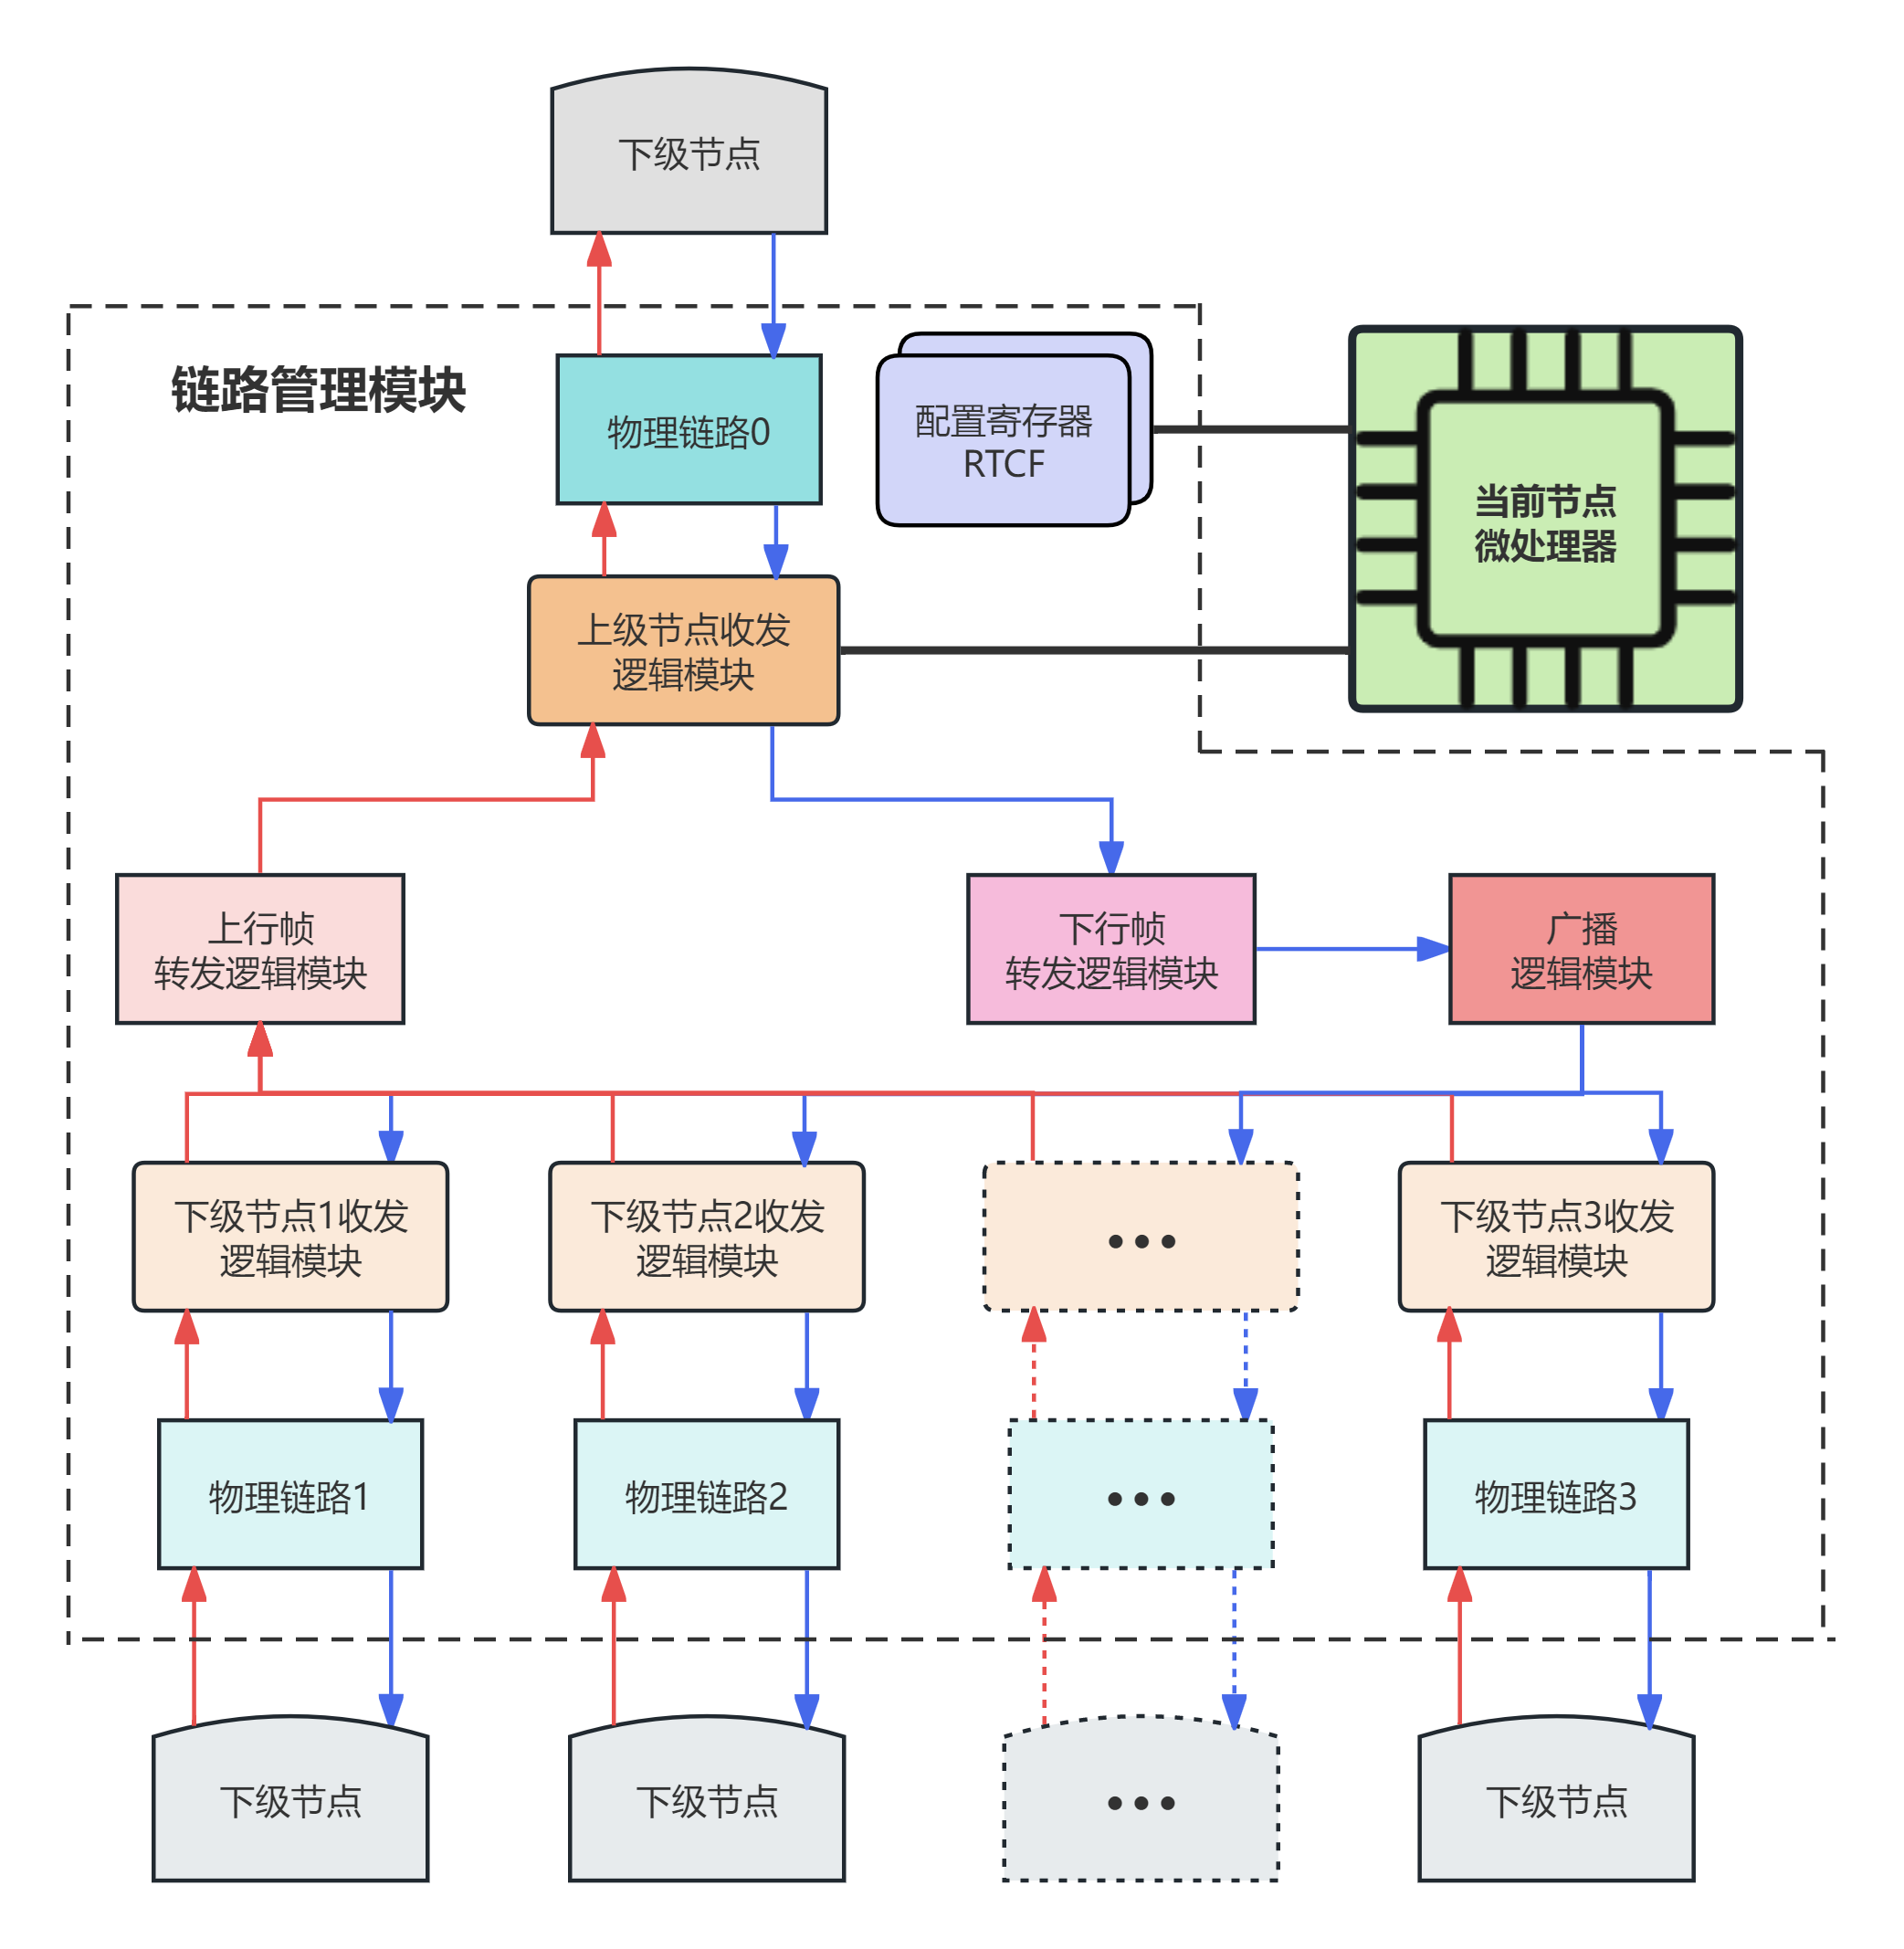
\includegraphics[width=1.0\linewidth]{rtmq/rtmq_link_module}
    \caption[链路管理模块内部逻辑结构图]{链路管理模块内部逻辑结构图\label{fig:rtmq_link_module}}
\end{figure}



\newpage
\section[章末小结]{章末小结}

测控系统在量子计算实验系统中占据着十分关键的位置,
为了满足量子计算发展过程中日益增高的测控需求,本章引入了一套强实时、可拓展、分布式的用于量子物理实验的实时微系统——RTMQ。RTMQ是专为量子物理实验设计的一套测控系统方案,它包含了一种专门设计的用于满足实时信息处理的微处理器架构以及配套的汇编指令集,此外还有服务于多节点拓展的实时通信链路系统。

本章首先明确了量子测控系统的两个主要挑战:信息处理实时性和大规模可拓展性,
随后介绍了RTMQ量子测控系统的整体架构以及每个RTMQ节点的内部模块。
接着描述了RTMQ微处理器所配套设计的汇编指令集,介绍了指令集的汇编指令格式以及其I类和A类两类指令的操作码、指令功能和编码方式,并给出了其时序控制结构实例。此外还介绍了RTMQ不同节点间的实时通信链路系统,该通信链路系统能够实现整个RTMQ节点树中不同节点的配置和时序同步,满足跨节点实时性的测控需求。

值得注意的是,从它的指令集中可以看到RTMQ测控系统是支持板上运算和信息处理的,这是与其它依靠时序发生器构成的测控系统本质不同的地方和优势所在。这些处理包括逻辑运算和算术运算,构成了一个微处理器。而RTMQ系统的微处理器从架构上与CPU有着本质的不同,虽然牺牲了些运算效率,RTMQ的数据处理是严格实时的。
这种RTMQ处理器架构同样也具有可拓展性和灵活性,我们可以方便地为它拓展和定义多种运算方式,也可以为其添加功能外设模块等,以适应更多更复杂任务的需求。对RTMQ量子测控系统的理解为后续设计测控板硬件及离子阱量子计算重要子系统的搭建和测试(第\ref{section:implementation}章)打下了基础。
